\documentclass{beamer}
\usetheme{Madrid}
\usecolortheme{default}

\usepackage[T1]{fontenc}
\usepackage[utf8]{inputenc}
\usepackage{amsmath,amssymb,bm,mathtools}
\usepackage{xcolor}
\usepackage{hyperref}
\usepackage{microtype}
\graphicspath{{./figures/}}
\usepackage{booktabs}

\title[Project 2]{Project 2}
\subtitle{CS 332, Fall 2025}
\author{Ben Cole \and Koshi Harashima}
\date{22 October, 2025}

\begin{document}

\maketitle

\section{Basic Setting}

\begin{frame}{Basic Setting \& Regret}
\textbf{Online learning setup}
\begin{itemize}
  \item $k$ actions, $n$ rounds; in round $i$ we choose $a_i$, then observe full payoffs $v_1^i,\dots,v_k^i\in[0,h]$ and obtain $v_{a_i}^i$.
  \item Algorithm payoff: $ALG=\sum_{i=1}^n v_{a_i}^i$; best-in-hindsight $OPT=\max_j \sum_{i=1}^n v_j^i$.
  \item Average regret: $\mathrm{Regret}_n=\frac{1}{n}(OPT-ALG)$.
\end{itemize}
\medskip
\textbf{Exponential Weights (EW)}
\[
\pi_j^i=\frac{(1+\epsilon)^{V_j^{i-1}/h}}{\sum_{j'}(1+\epsilon)^{V_{j'}^{i-1}/h}},\quad
V_j^{i}=\sum_{r=1}^{i}v_j^r
\]
\textbf{Bound:} $\mathrm{Regret}_n\le \epsilon n h+\frac{h\log k}{\epsilon}$; optimal $\epsilon=\sqrt{\frac{\log k}{n}}$ gives $2h\sqrt{n\log k}$.
\end{frame}

\begin{frame}{EW: Rates \& Monte Carlo Setup}
\textbf{Learning rates compared}
\begin{itemize}
  \item No learning: $\epsilon\approx 0$ (uniform random).
  \item Theoretical: $\epsilon=\sqrt{\ln k / n}$.
  \item FTL: $\epsilon\to\infty$ (or explicit Follow-The-Leader).
\end{itemize}
\textbf{MC trials}
\begin{itemize}
  \item Fix $k=5$, $n=1000$; multiple runs; report mean regret with confidence intervals.
  \item Evaluate two models: Adversarial Fair Payoffs (AFP) and Bernoulli Payoffs (BP).
\end{itemize}
\end{frame}

\section{Part 1}

\begin{frame}{Part 1 - Summary}
\textbf{Methods}\\
In AFP and BP, we first gain intuition from observation, then simulate them.

\vspace{0.7em}
\textbf{Results}\\
In AFP, FTL works poorly, while other learning rates work well. In BP, FTL works better than the others.

\vspace{0.7em}
\textbf{Takeaways}\\
FTL performs best when there is an optimal arm (stationary). Random and optimal learning rates perform best without a stable optimal arm.
\end{frame}

\subsection{A: AFP}

\begin{frame}{Part 1A (AFP): Setting \& Intuition}
\textbf{Setting}
\begin{itemize}
  \item Each round: draw $x\sim U[0,1]$; assign to arm $j^*=\arg\min_j V_{j}^{i-1}$ (others get $0$).
  \item Fixed: $k=5$, $n=1000$.
\end{itemize}
\textbf{Intuition}
\begin{itemize}
  \item FTL chases the leader and is “punished” next round $\Rightarrow$ regret grows roughly linearly.
  \item Random or theoretical $\epsilon$ avoid overreaction $\Rightarrow$ near-zero regret.
\end{itemize}
\centering
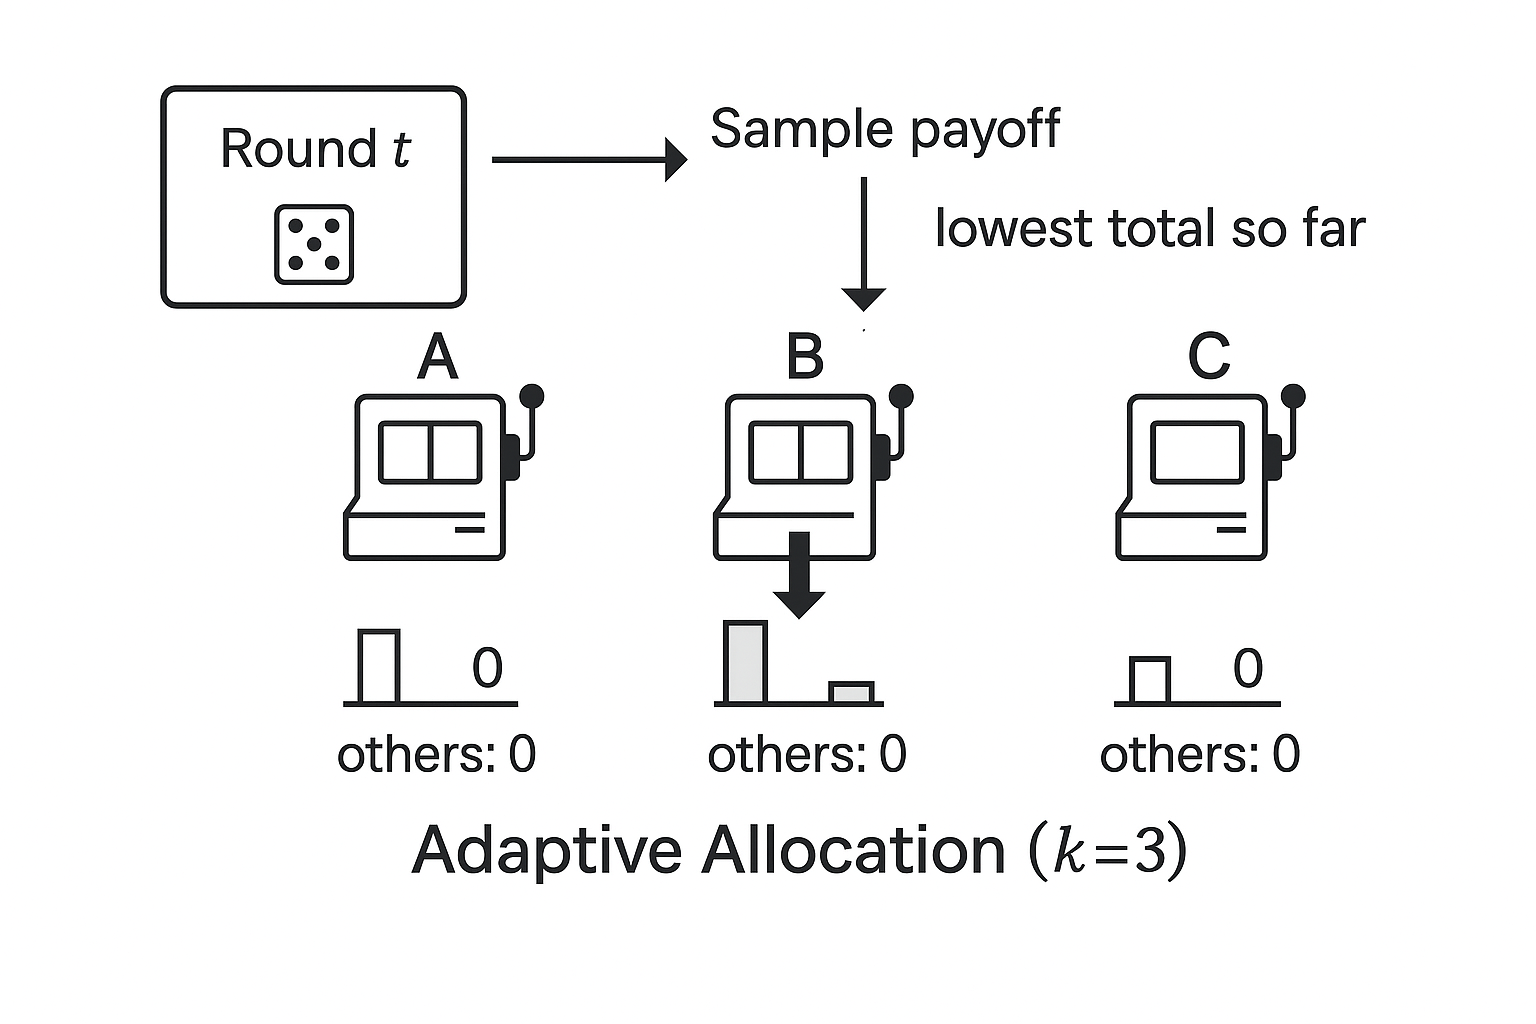
\includegraphics[width=0.45\textwidth]{../figures/Image_A.png}
\end{frame}

\begin{frame}{Part 1A: Results}
\begin{columns}[T,onlytextwidth]
  \column{0.5\textwidth}
  \centering
  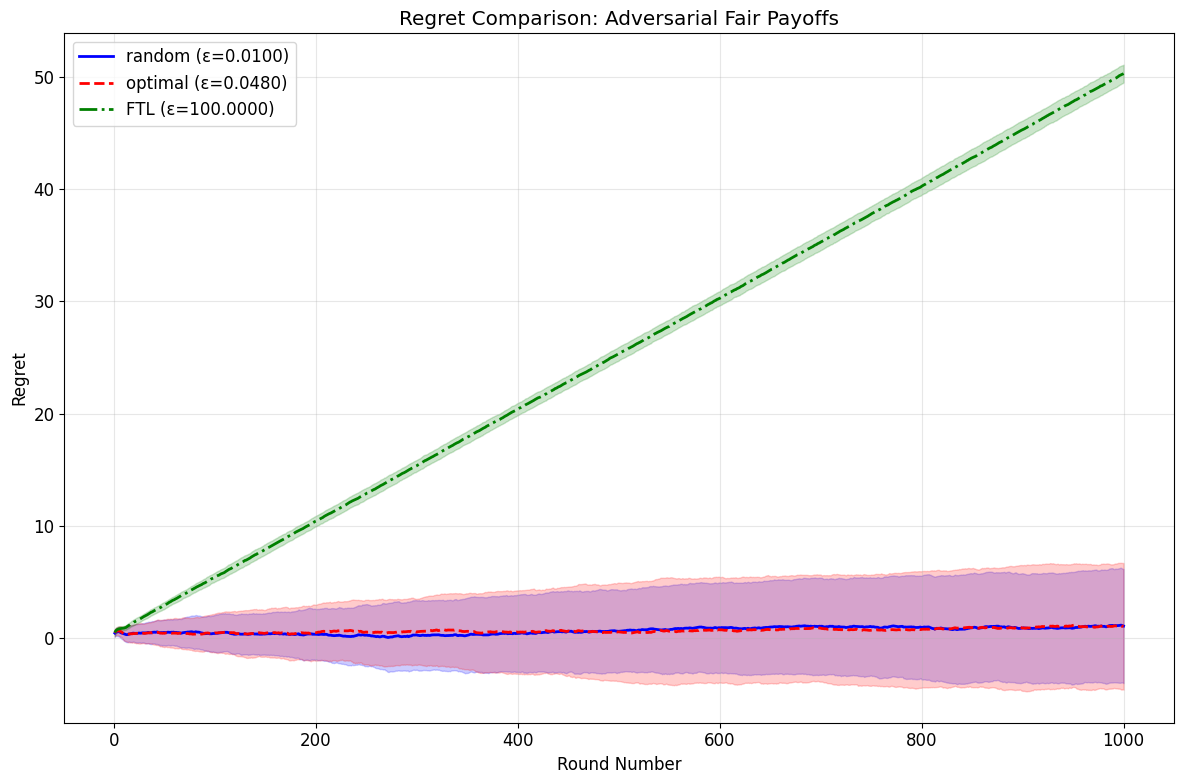
\includegraphics[width=\linewidth]{../figures/AFR_regret.png}

  \column{0.5\textwidth}
  \centering
  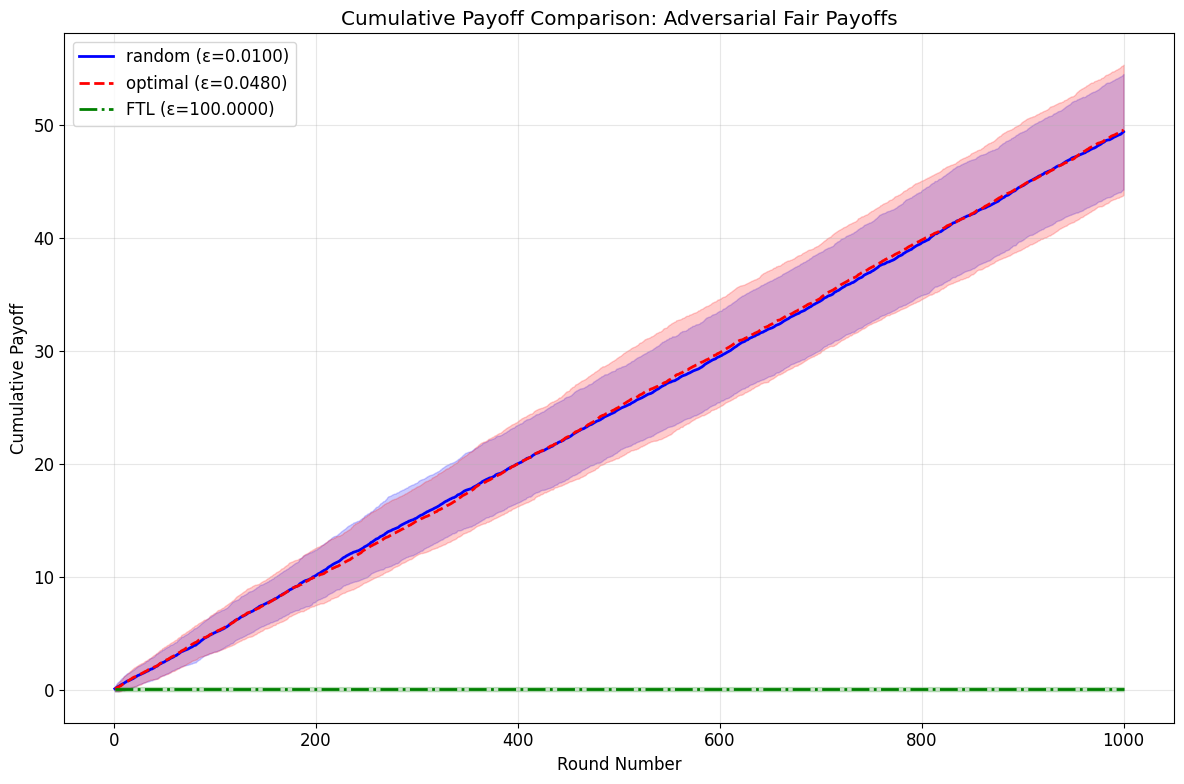
\includegraphics[width=\linewidth]{figures/AFR_payoff.png}
\end{columns}
\vspace{0.3em}
\small \textit{Note:} With $\epsilon=\sqrt{\ln k/n}$, the bound is $\approx 110$ for $h=1,k=5,n=1000$; observed regret stays below this.
\end{frame}

\subsection{B : BP}

\begin{frame}{Part 1B (BP): Setting \& Intuition}
\textbf{Setting}
\begin{itemize}
  \item Fix $p_j\in[0,1/2]$; each round $v_j^i\sim \mathrm{Bernoulli}(p_j)$; full information.
  \item $k=5$, $n=1000$.
\end{itemize}
\textbf{Intuition}
\begin{itemize}
  \item Stationary environment with a best arm $\Rightarrow$ FTL quickly locks in and achieves low regret.
  \item Random / theoretical $\epsilon$ explore more and lag.
\end{itemize}
\centering
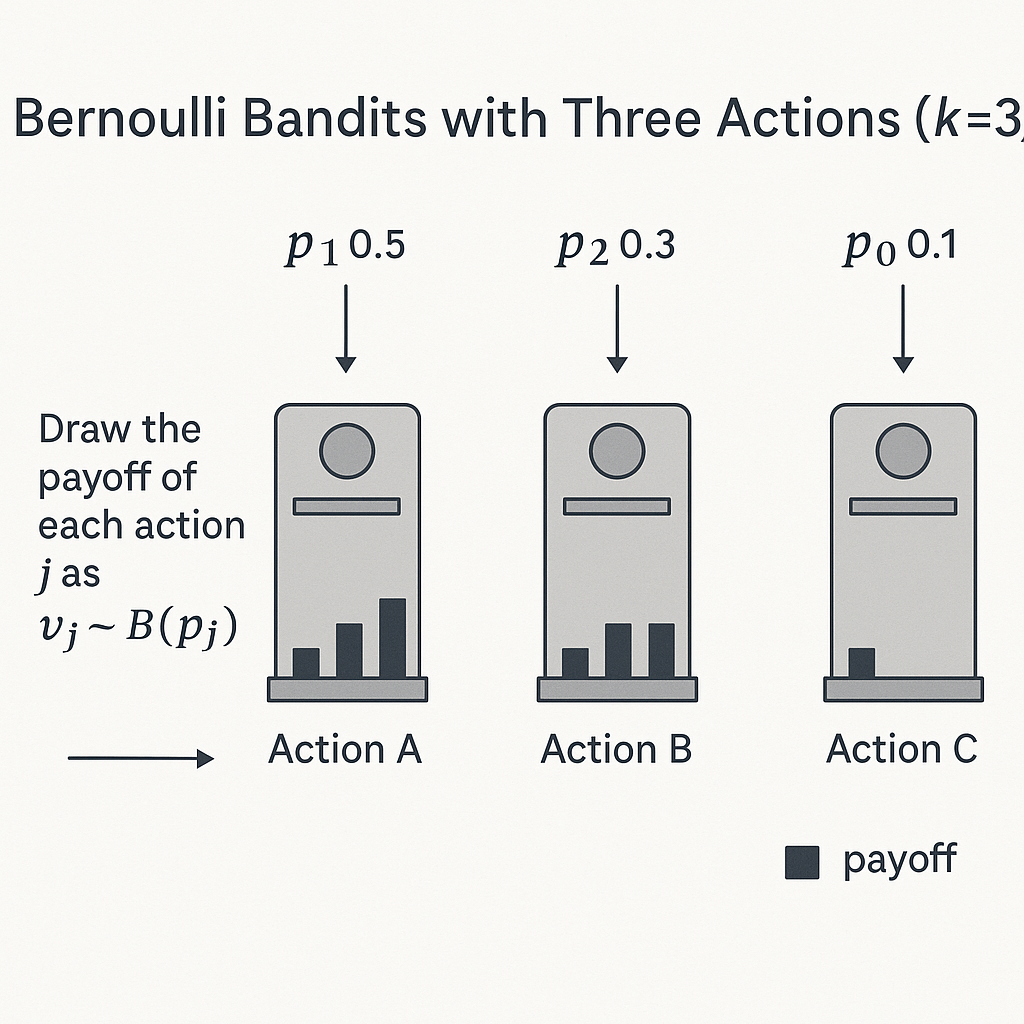
\includegraphics[width=0.4\textwidth]{../figures/Image_B.png}
\end{frame}

\begin{frame}{Part 1B: Results}
\begin{columns}[T,onlytextwidth]
  \column{0.5\textwidth}
  \centering
  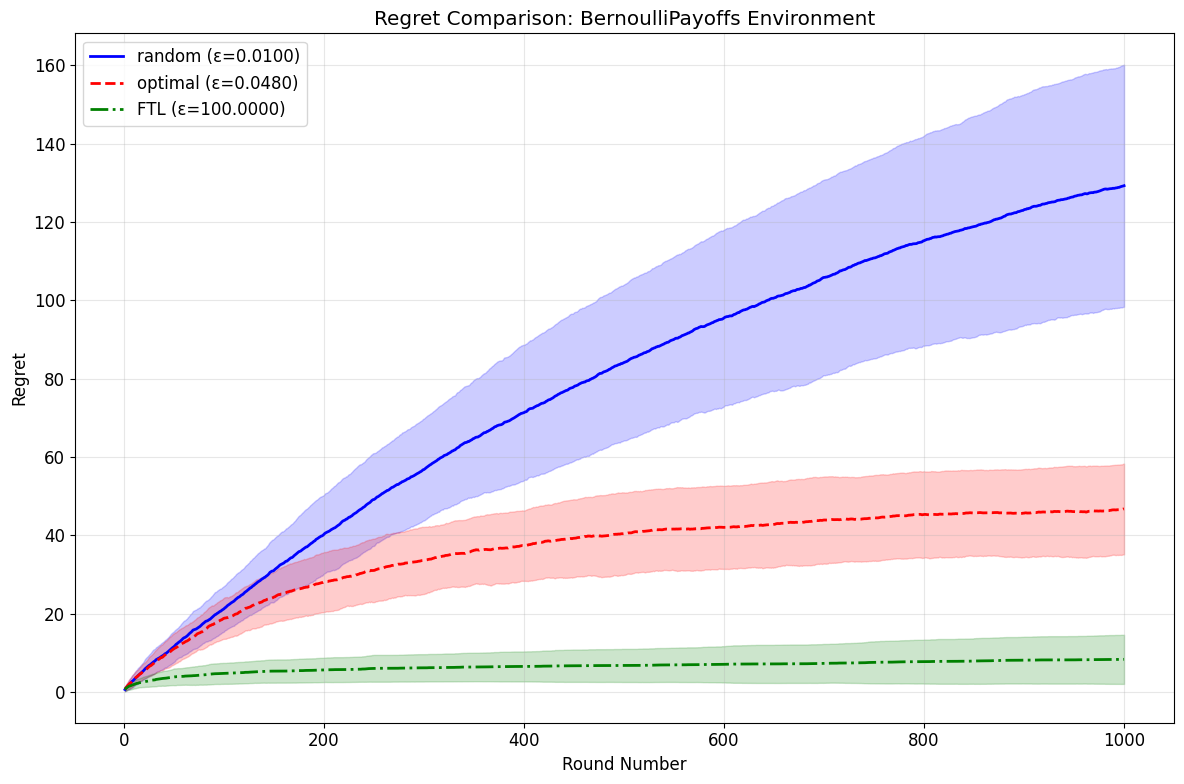
\includegraphics[width=\linewidth]{../figures/BP_regret.png}

  \column{0.5\textwidth}
  \centering
  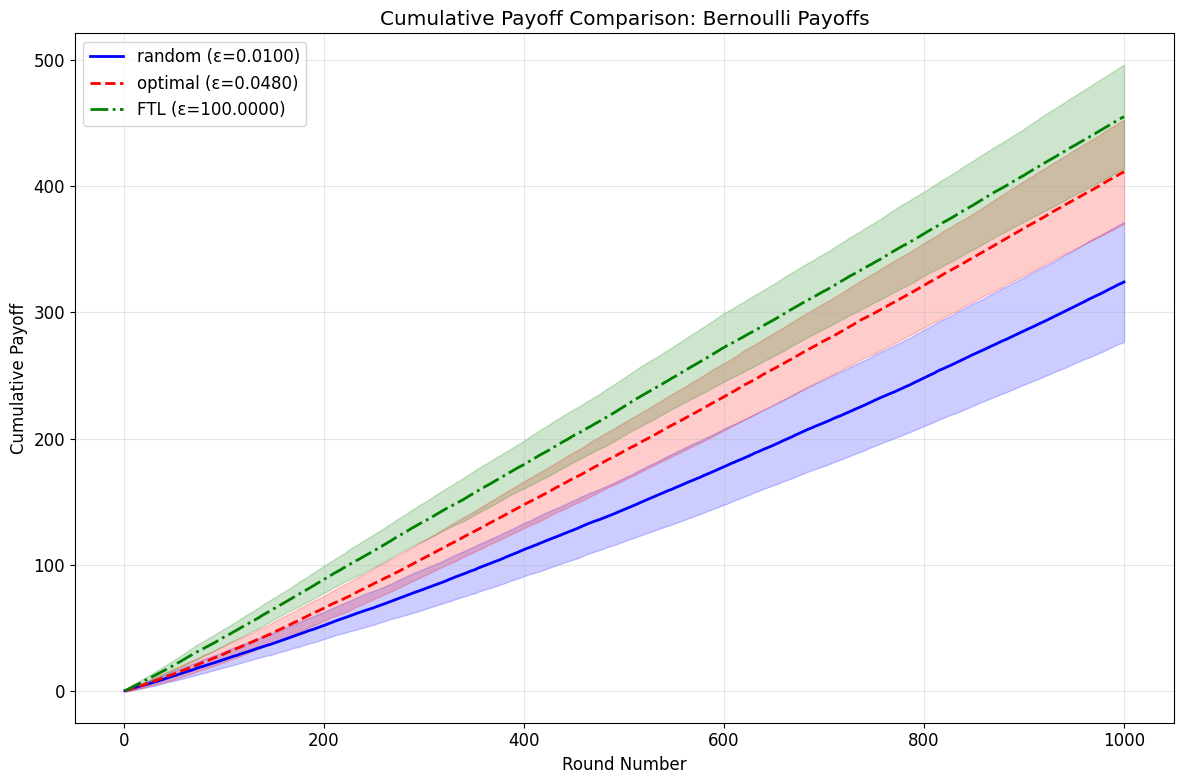
\includegraphics[width=\linewidth]{figures/BP_payoff.png}
\end{columns}
\vspace{0.3em}
\small \textit{Note:} Same theoretical ceiling applies; empirically FTL is best here.
\end{frame}

\section{Part 2}

% ---------- C (MERGED) ----------
\subsection{C : PP}

\begin{frame}{Part 2C (Pachinko): Methods, Data \& Intuition}
\textbf{Methods}
\begin{itemize}
  \item Treat each store as an arm; daily ROI normalized to $[0,1]$; full information.
  \item Four Tokyo stores; nonstationary ROI due to store setting changes.
\end{itemize}
\textbf{Intuition}
\begin{itemize}
  \item FTL (follow past best store) works if ROI drifts slowly.
\end{itemize}
\centering
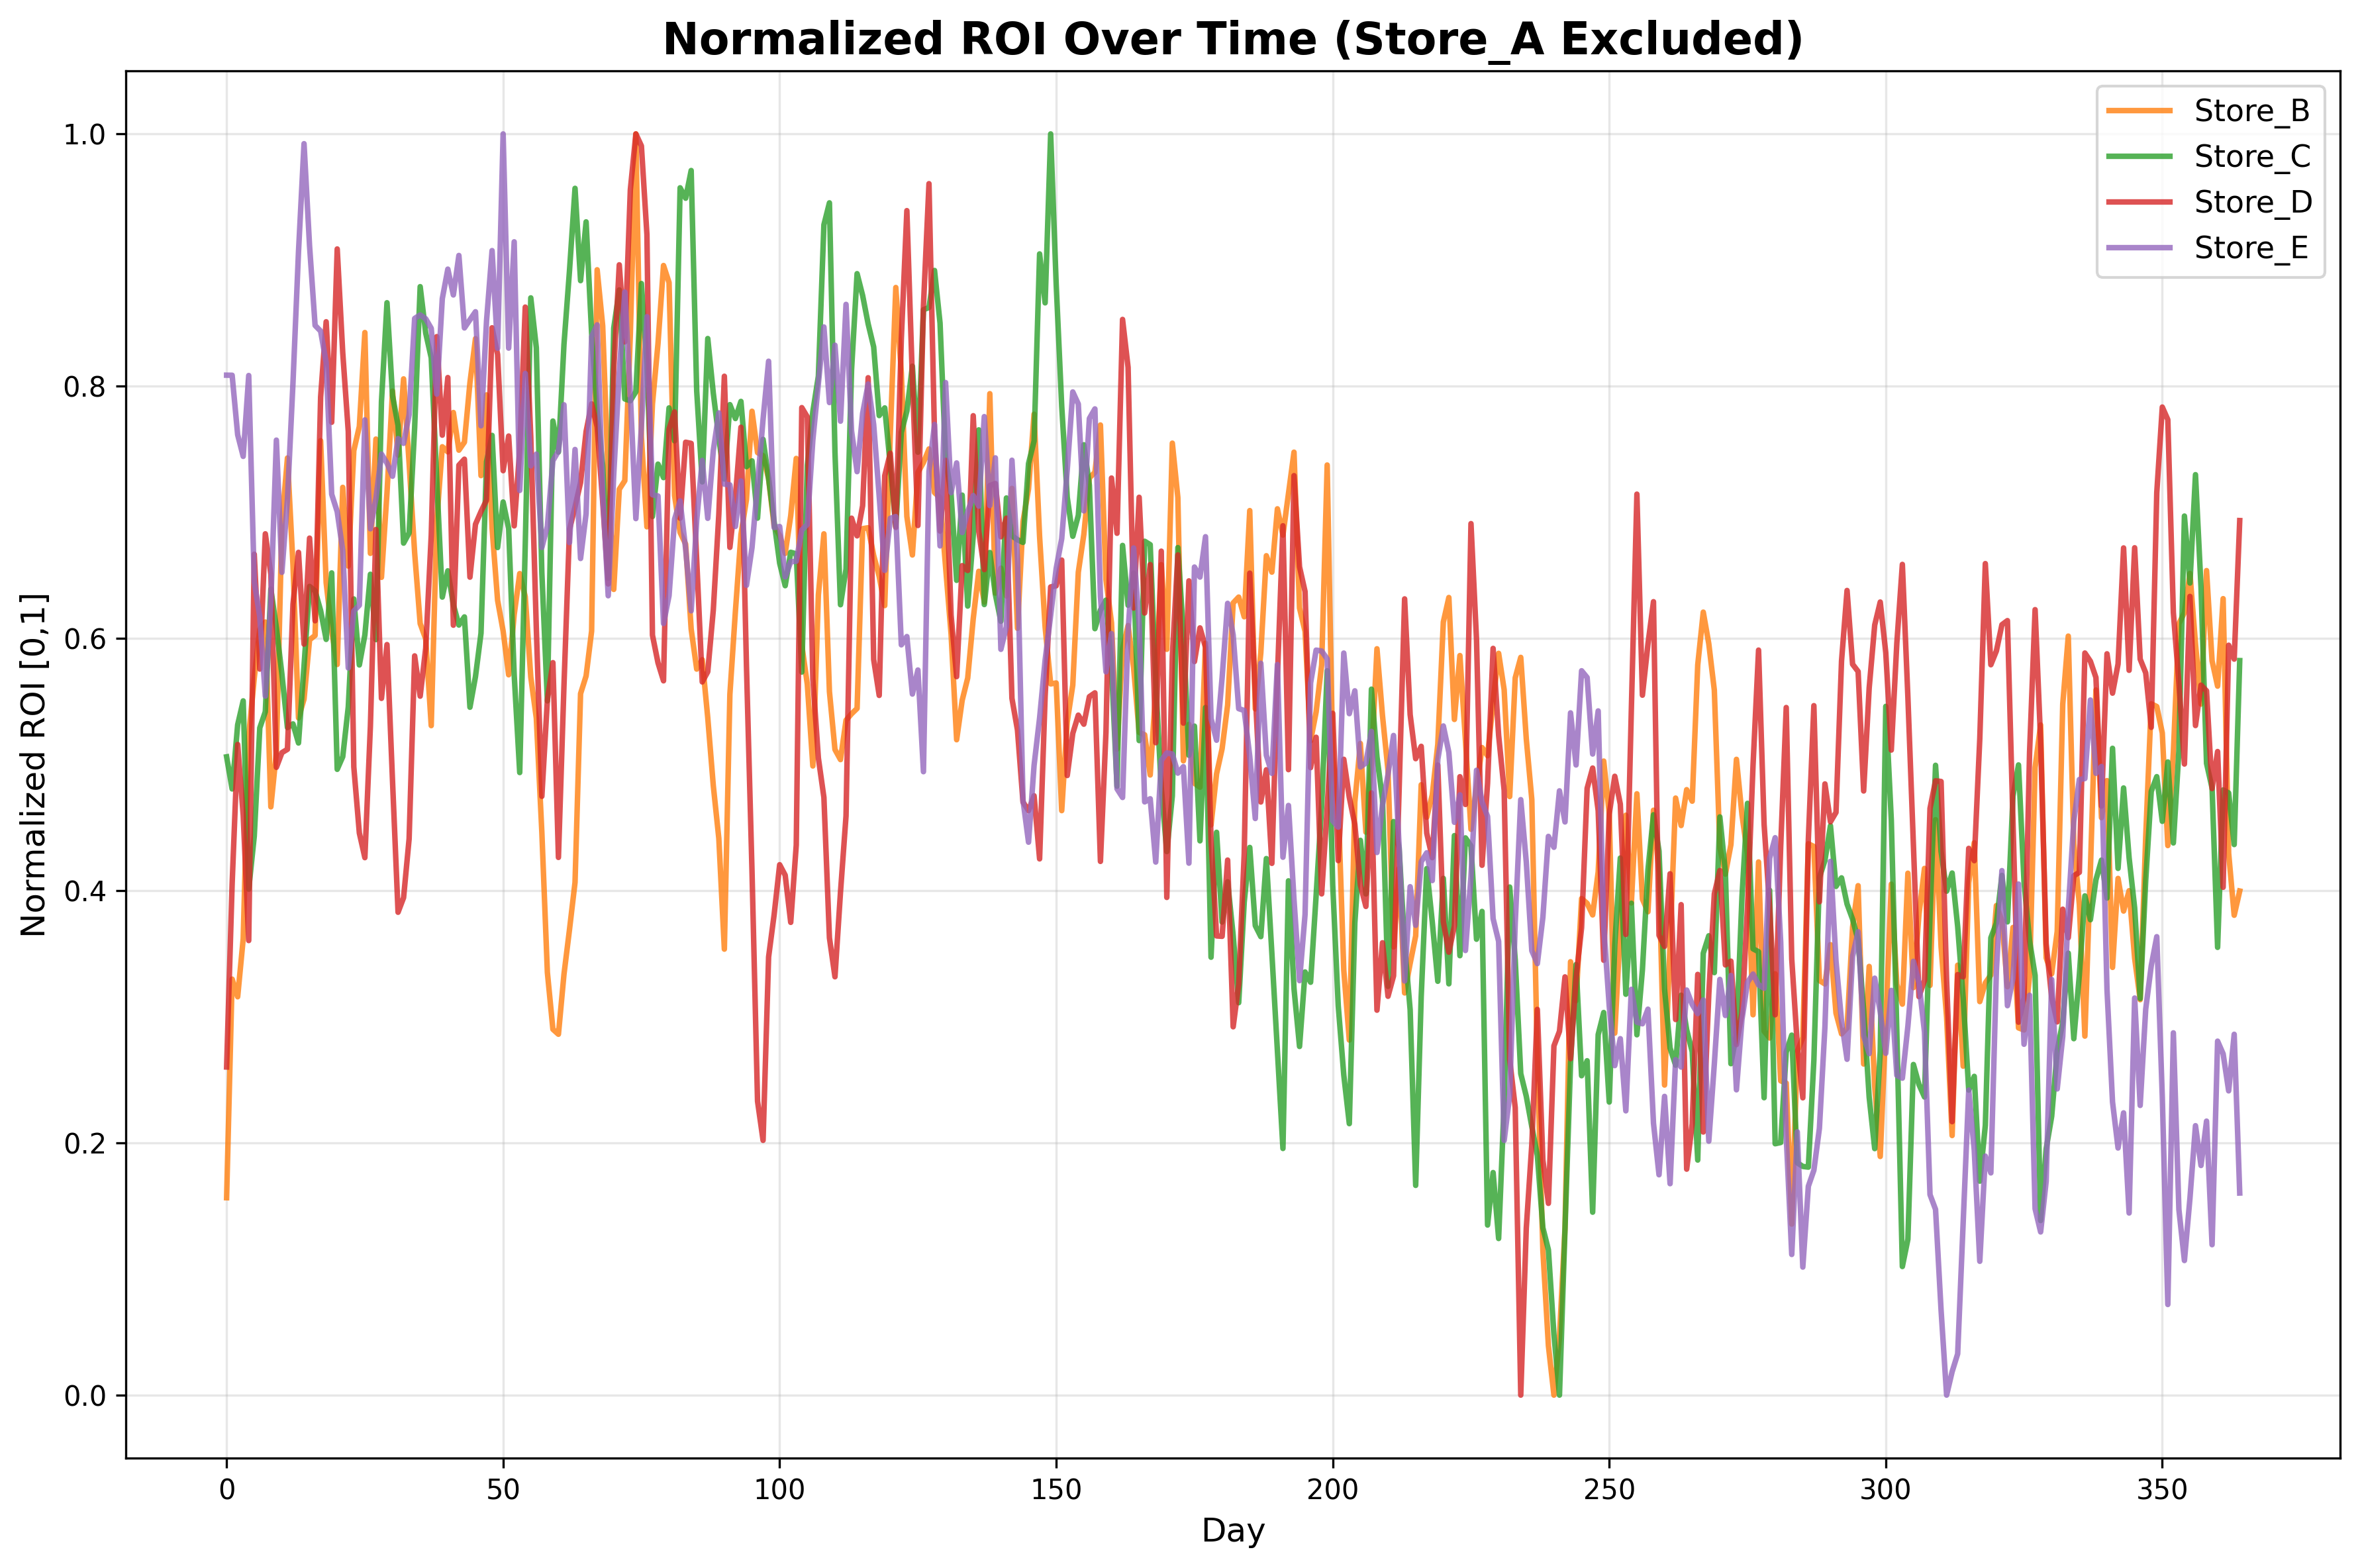
\includegraphics[width=0.65\textwidth]{332Project2/figures/PP_data_timeseries_store_A_excluded.png}
\end{frame}

\begin{frame}{Part 2C: Results}
\begin{columns}[T,onlytextwidth]
  \column{0.5\textwidth}
  \centering
  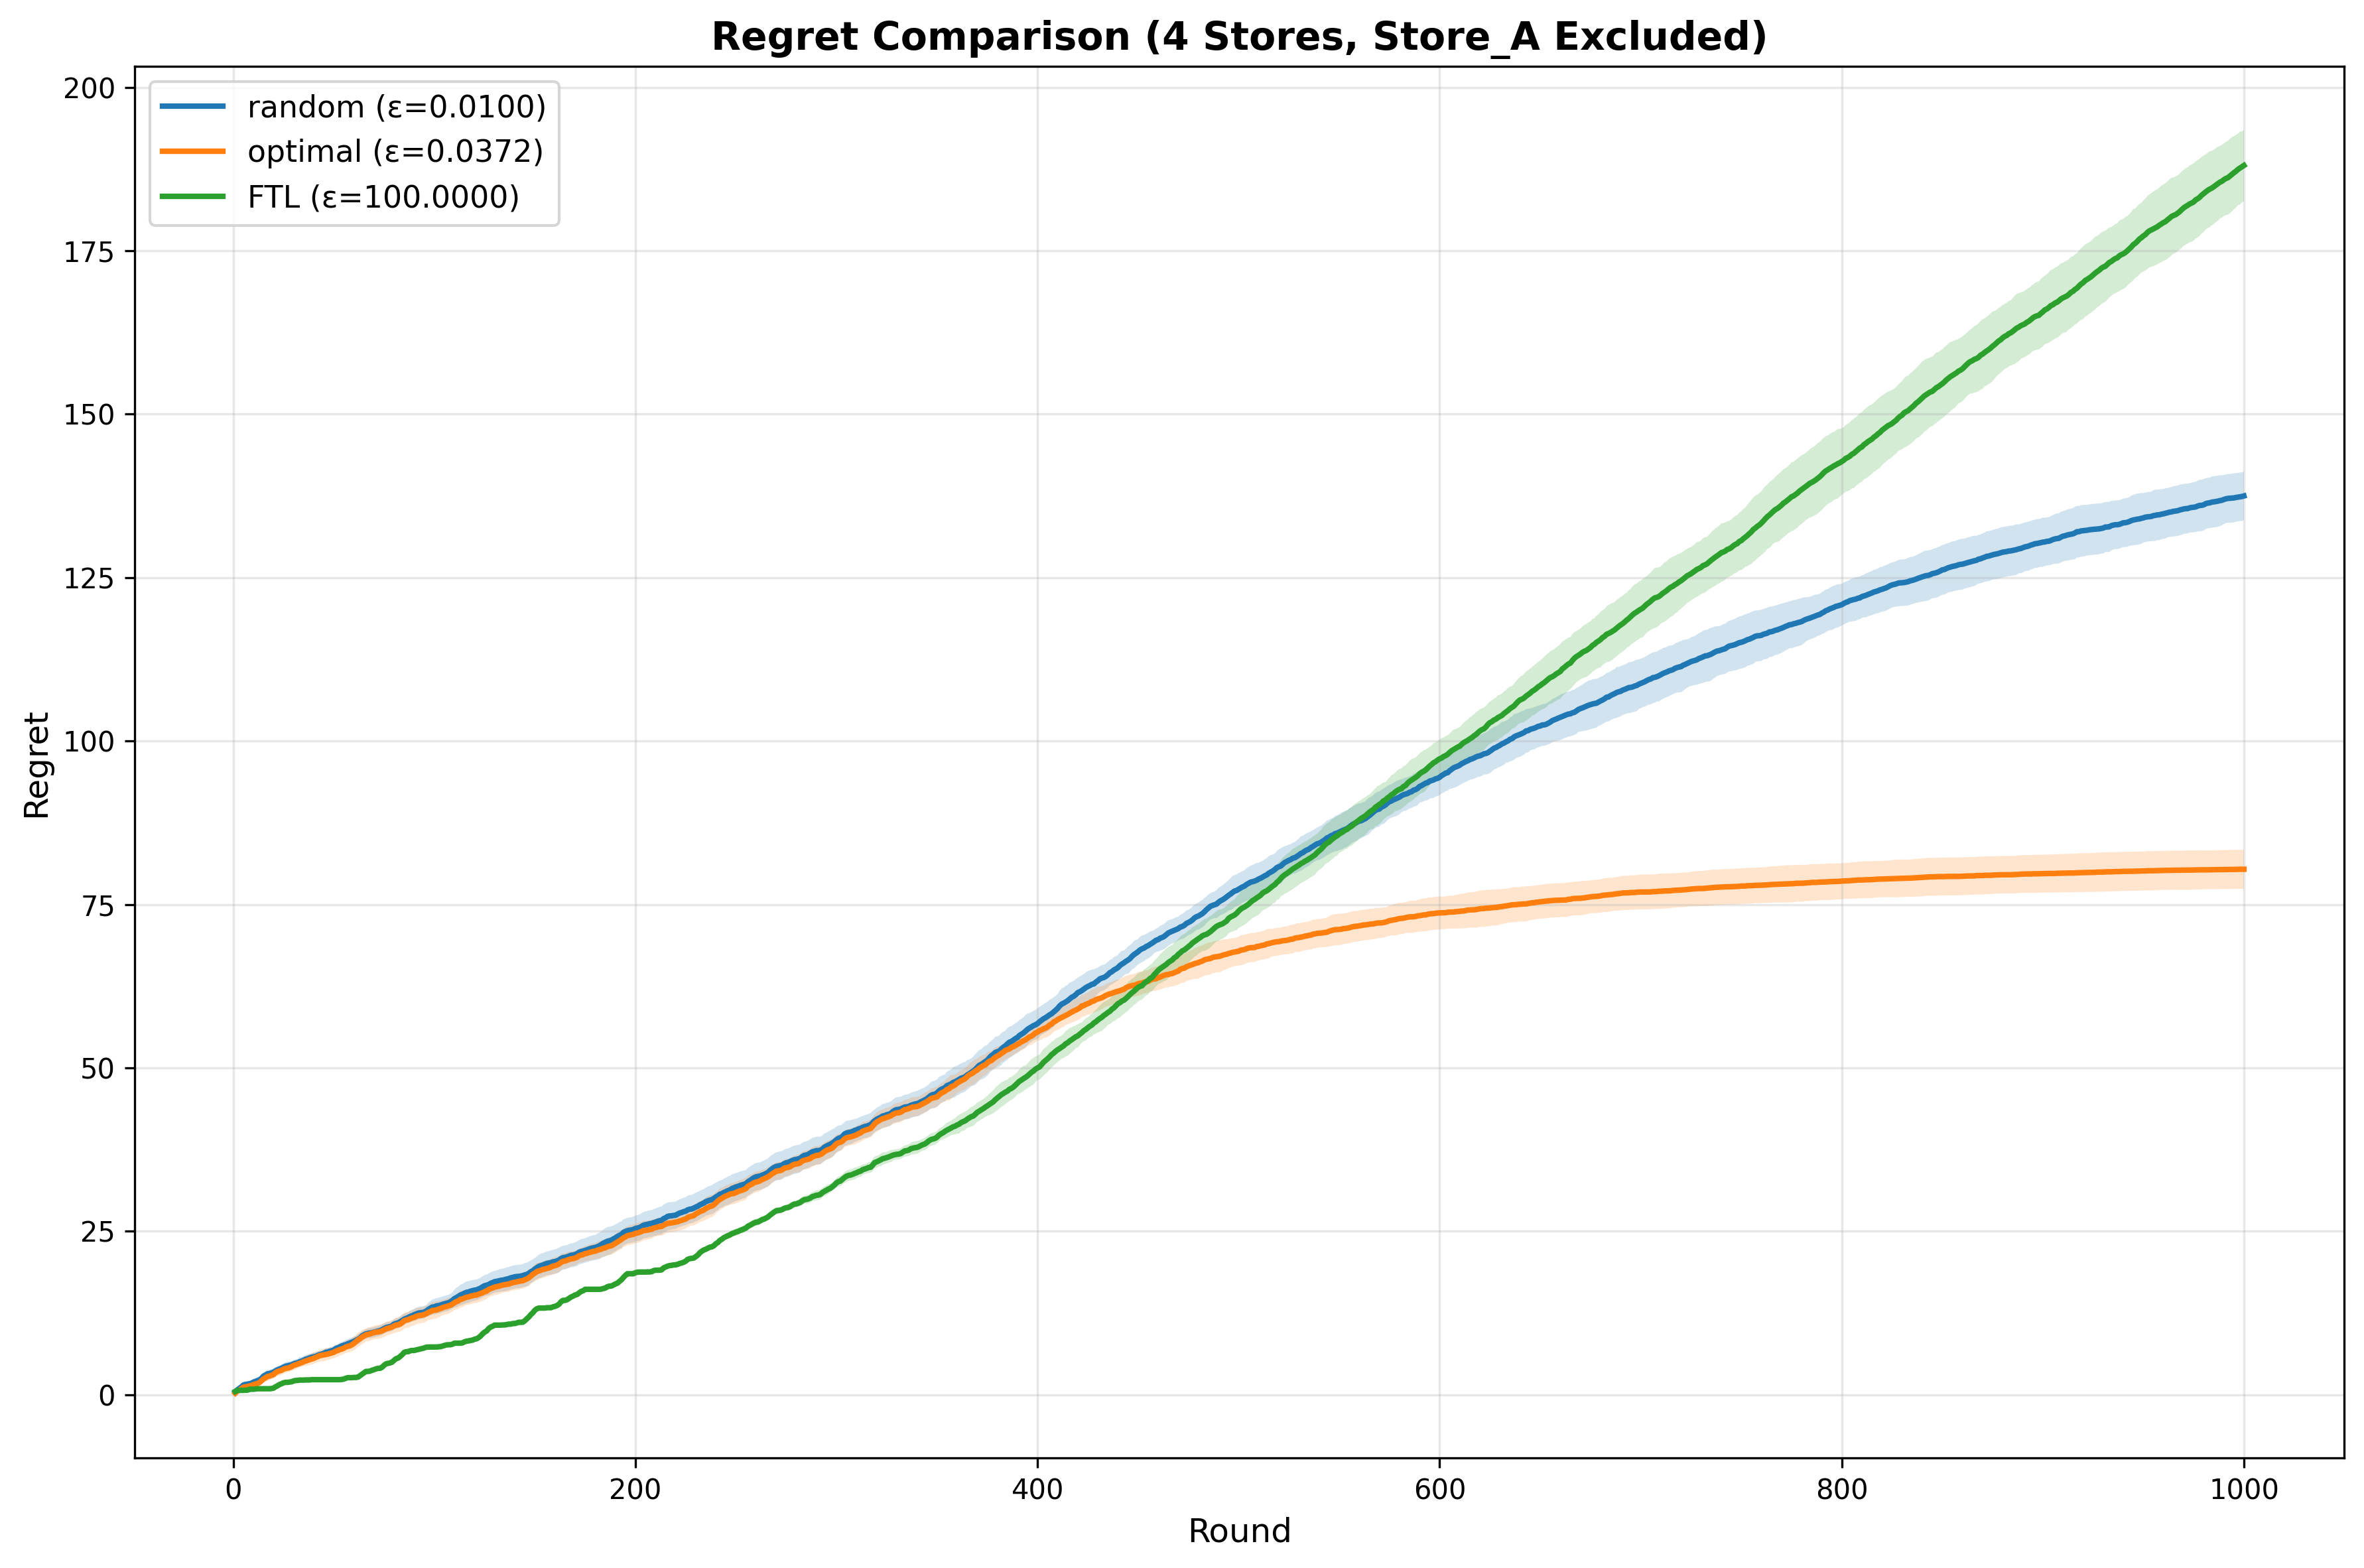
\includegraphics[width=\linewidth]{332Project2/figures/PP_regret.png}

  \column{0.5\textwidth}
  \centering
  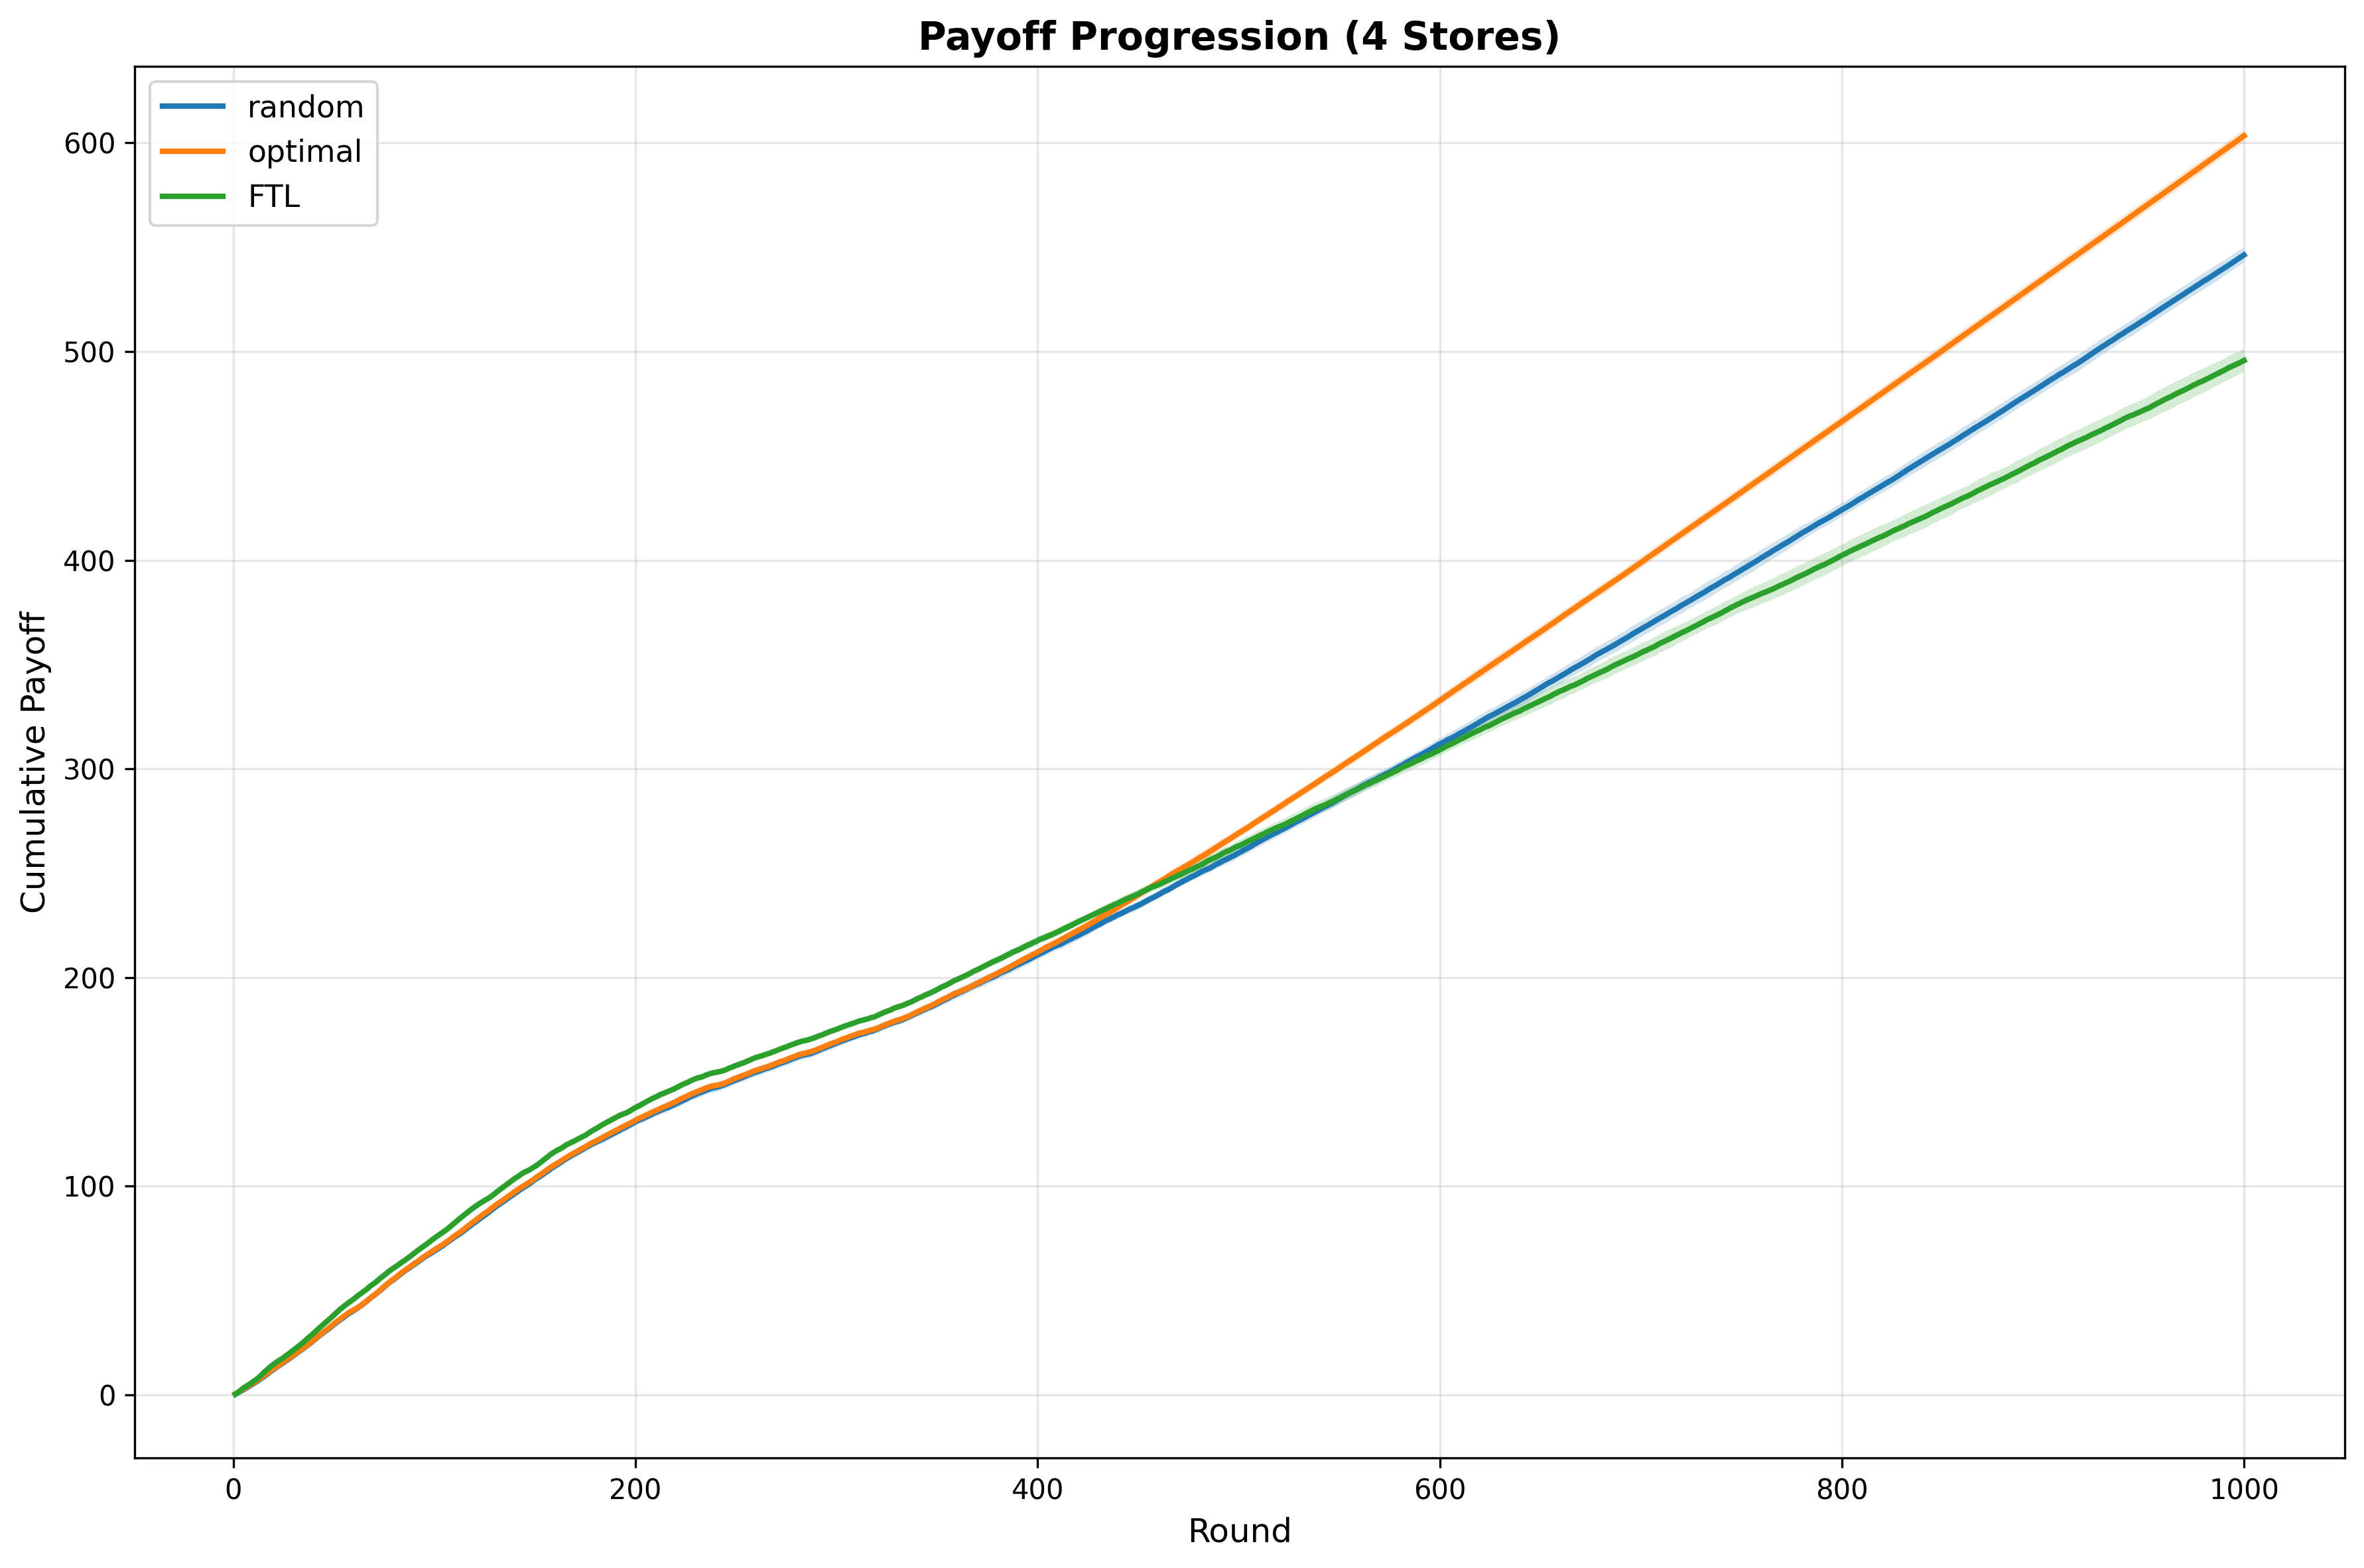
\includegraphics[width=\linewidth]{332Project2/figures/PP_payoff.png}
\end{columns}
\end{frame}

\subsection{D : RP}

\begin{frame}{D - Setting}
    Here is our model in Part D. I model the environment in which researcher search the previous research papers for his work.\\
    In each round i, 
    \begin{itemize}
        \item There is hidden(unobserved) regime 
        \item The researcher observes the clusters and the origin of the clusters of candidate papers 
        \item The researcher chooses an \textbf{effort allocation vector}
              \[
              w_t = (w_{t,1}, \ldots, w_{t,k}), 
              \quad \text{such that } \sum_{j=1}^{k} w_{t,j} = 1,\; w_{t,j} \ge 0.
              \]
        \item The payoff is computed as a linear combination:
              \[
              U_t = \alpha_t^{\mathsf{T}} w_t.
              \]
    \end{itemize}
\end{frame}

\begin{frame}{D - Techniques}
    In academic world, there are two often-said characteristics
    \begin{itemize}
        \item \textbf{High-quality papers are mass-produced by a cluster of researchers}
        \begin{itemize}
            \item we can formulate this by introducing correlation of paper's value in a cluster
            \item which disturbs uniform guessing to be optimal and to converge to the no-regret
        \end{itemize}
        \item \textbf{Frequent innovations (regime changes) in research methods}
        \begin{itemize}
            \item we can formulate this by introducing possibility of regime changes 
            \item which disturbs FTL to be optimal and to converge to the no-regret
        \end{itemize}
    \end{itemize}
    Our technique leverages these well-known properties to formulate online learning in a way that suits the conditions of our problem.
\end{frame}

\begin{frame}{D - Game structure and Intuition}
Here's our intuition:
\begin{itemize}
    \item FTL and uniform guessing will both work similarly to typical behaviors of researchers in the real world who choose the leading university (FTL) or collect from any/all universities (uniform random guessing).
    \item Between FTL and random guessing, maybe there is an optimal learning rate
\end{itemize}
\end{frame}

\begin{frame}{D - Results (Regrets)}
\begin{figure}
    \centering
    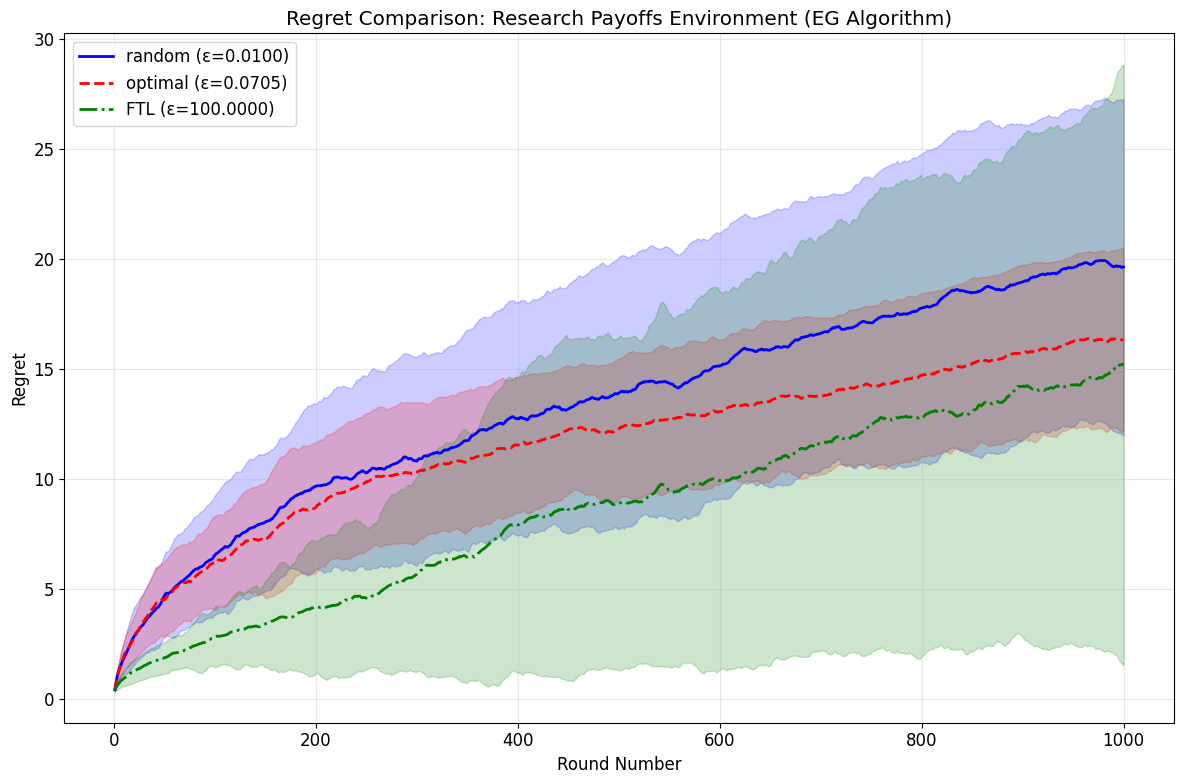
\includegraphics[width=0.8\linewidth]{332Project2/figures/RP_regret.png}
    \caption{Regret}
    \label{fig:placeholder}
\end{figure}
\end{frame}

\begin{frame}{D - Results (Payoffs)}
\begin{figure}
    \centering
    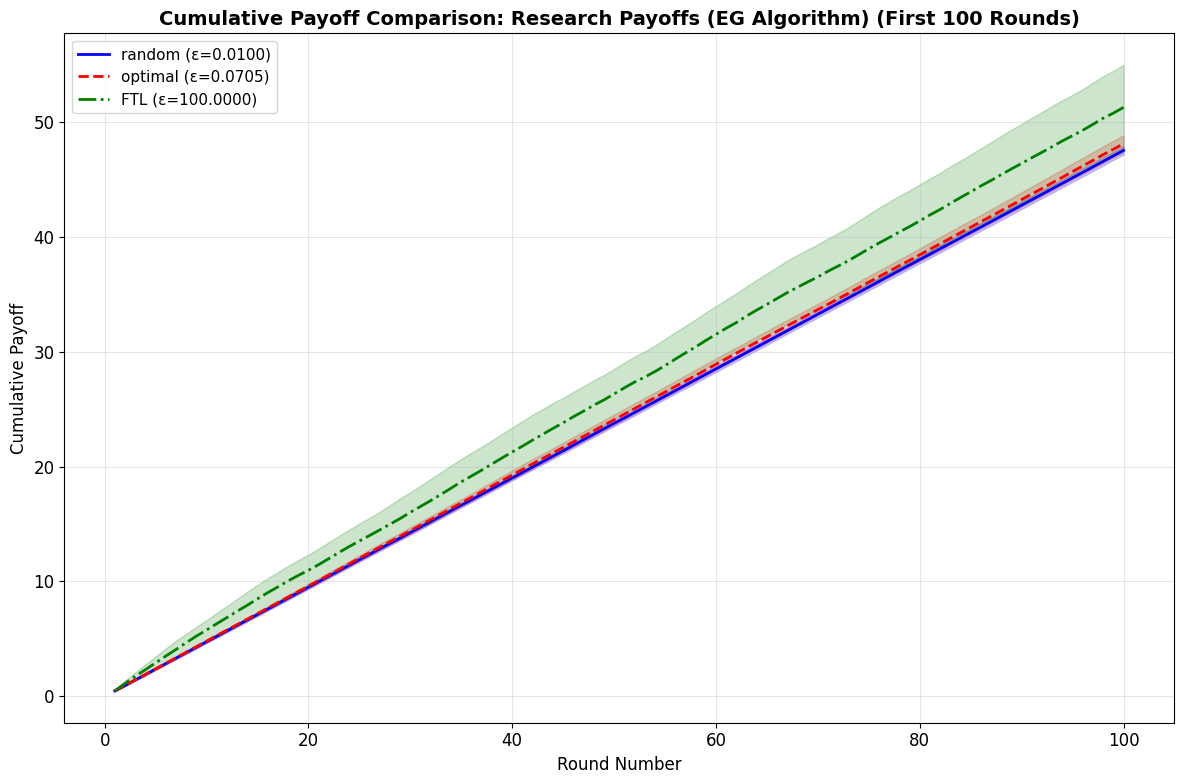
\includegraphics[width=0.8\linewidth]{332Project2/figures/RP_payoff.png}
    \caption{Payoff}
    \label{fig:placeholder}
\end{figure}
\end{frame}


\section{Reference and Usage of AI}

\begin{frame}{Reference and Usage of AI}
\begin{itemize}
    \item \textbf{Pachinko store data:} Daily store-level ``balls in/out'' statistics obtained from \emph{SloRepo} (\url{https://slorepo.com}). Data accessed on October 22, 2025 (America/Chicago).
    \item AI assistance was used for coding and figure generation; final verification, interpretation, and responsibility rest with the authors.
\end{itemize}
\end{frame}

\section{Appendix}
\begin{frame}{D - Appendix(Model)}
\begin{itemize}
    \item The research world is divided into several \textbf{clusters of researchers} 
          (e.g., MIT, Stanford, Northwestern).
    \item Each cluster represents a correlated set of ideas or papers whose values
          move together (\textbf{intra-cluster correlation}).
    \item At every round, the researcher distributes total effort 
          across candidate papers:
          \[
          \sum_{i=1}^{N} w_{i,t} = 1, \quad w_{i,t} \ge 0.
          \]
    \item The payoff is the weighted sum of paper values:
          \[
          U_t = \alpha_t^{\mathsf{T}} w_t.
          \]
\end{itemize}
\end{frame}

\begin{frame}{D - Appendix{Model}}
    \begin{block}{Regime Dynamics}
    \begin{itemize}
        \item At any time, one cluster becomes \textbf{hegemony} (high valuation).
        \item The dominant cluster changes according to a \textbf{Markov transition} with probability p:\\
        for example, p = 0.7, 
              \[
              \Pr(z_t = z_{t-1}) = 0.7, \quad 
              \Pr(z_t \neq z_{t-1}) = 0.3.
              \]
        \item In each regime:
              \begin{itemize}
                  \item One cluster has \textbf{High values} ($[0.7, 1.0]$)
                  \item Another has \textbf{Middle values} ($[0.5, 0.8]$)
                  \item Others remain \textbf{Low values} ($[0.0, 0.4]$)
              \end{itemize}
    \end{itemize}
    \end{block}
\end{frame}


\begin{frame}{D - Appendix (Example)}
\scriptsize
\textbf{Example Setting}
    \begin{itemize}
        \item Imagine three major research clusters:
              \textbf{MIT}, \textbf{Stanford}, and \textbf{Northwestern}.
        \item Each cluster represents a group of researchers 
              whose papers are highly correlated in value (citations, attention, or impact).
        \item The researcher (our agent) allocates research effort
              across papers from these clusters every round.
    \end{itemize}
\textbf{Regime-Dependent Dominance}
\begin{itemize}
        \item At one period, the \textbf{MIT cluster} becomes dominant 
              --- its papers are cited frequently, gaining high valuation.
        \item Over time, attention shifts:
              Stanford’s ideas rise in popularity,
              then Northwestern takes the lead.
        \item These shifts occur through a stochastic 
              \textbf{Markov regime transition}, 
              creating a dynamic environment.
    \end{itemize}
\textbf{Researcher’s Behavior}
\begin{itemize}
        \item In each round, the researcher chooses how to distribute effort:
              \[
              w_t = (w_{\text{MIT}}, w_{\text{Stanford}}, w_{\text{Northwestern}}),
              \quad \sum w_t = 1.
              \]
        \item The payoff is the weighted performance of papers:
              \[
              U_t = \alpha_t^{\mathsf{T}} w_t.
              \]
        \item As the dominant cluster changes, the researcher must 
              continuously reallocate effort to follow the new trend.
\end{itemize}
\end{frame}

\begin{frame}{D- Appendix (Algorithm in the real world)}
\scriptsize
\textbf{1. Follow-The-Leader (FTL)}
    \begin{itemize}
        \item \textbf{Intuitive meaning:}
              \begin{itemize}
                  \item “MIT is the most famous and successful group — 
                        just follow their papers.”
                  \item Represents a researcher who always trusts 
                        the cluster that has performed best in the past.
              \end{itemize}
        \item \textbf{Problem:} 
              When regimes shift (e.g., attention moves from MIT to Stanford),
              FTL reacts too slowly and suffers large regret.
    \end{itemize}
\textbf{2. Uniform Guessing}
    \begin{itemize}
        \item \textbf{Intuitive meaning:}
              \begin{itemize}
                  \item “Every cluster might have something interesting —
                        I’ll pick papers at random.”
                  \item Represents an exploratory but non-learning researcher.
              \end{itemize}
        \item \textbf{Problem:} 
              Ignores structure and fails to exploit high-performing clusters.
    \end{itemize}
\textbf{Summary about Algorithms}
    \begin{itemize}
        \item Both FTL and Uniform Guessing resemble 
              intuitive human search behaviors in academia.
        \item FTL overfits to the past (conservative imitation),
              while Uniform Guessing underfits (pure exploration).
    \end{itemize}
\end{frame}

\begin{frame}{D - Appendix(Compare EG and EW)}
\textbf{Extension}
    \begin{itemize}
        \item The \textbf{Exponential Weights (EW)} algorithm updates 
              a probability vector over discrete actions:
              \[
              w_{t+1,i} 
              = 
              \frac{
                  w_{t,i} \exp(\varepsilon \alpha_{t,i})
              }{
                  \sum_{j=1}^{k} w_{t,j} \exp(\varepsilon \alpha_{t,j})
              }.
              \]
        \item EW assumes a \textbf{finite action set} and interprets weights as probabilities.
    \end{itemize}
\textbf{Exponentiated Gradient (EG)}
    \begin{itemize}
        \item EG generalizes EW to an \textbf{$N$-dimensional continuous decision space}.
        \item The parameter vector $w_t \in \Delta^N$ represents 
              a continuous allocation (effort, attention, or resource):
              \[
              w_{t+1}
              = 
              \frac{
                  w_t \odot \exp(\varepsilon \nabla_t)
              }{
                  \|\,w_t \odot \exp(\varepsilon \nabla_t)\|_1
              },
              \quad
              \nabla_t = \alpha_t = \frac{\partial U(w_t)}{\partial w_t}.
              \]
    \end{itemize}
\end{frame}

\end{document}